% This example is meant to be compiled with lualatex or xelatex
% The theme itself also supports pdflatex
\PassOptionsToPackage{unicode}{hyperref}
\documentclass[aspectratio=1610, 12pt, xcolor=dvipsnames]{beamer}

% Warning, if another latex run is needed
% \usepackage[aux]{rerunfilecheck}

% just list chapters and sections in the toc, not subsections or smaller
\setcounter{tocdepth}{1}

%------------------------------------------------------------------------------
%------------------------------ Fonts, Unicode, Language ----------------------
%------------------------------------------------------------------------------
\usepackage{fontspec}
\defaultfontfeatures{Ligatures=TeX}  % -- becomes en-dash etc.

% german language
\usepackage{polyglossia}
\setdefaultlanguage{german}

% for english abstract and english titles in the toc
\setotherlanguages{english}

% intelligent quotation marks, language and nesting sensitive
\usepackage[autostyle]{csquotes}

% microtypographical features, makes the text look nicer on the small scale
\usepackage{microtype}

% colors and stuff
\usepackage{xcolor}
\usepackage[most]{tcolorbox}
\tcbset{on line, 
        boxsep=4pt, left=0pt,right=0pt,top=0pt,bottom=0pt,
        colframe=white,colback=SpringGreen,  
        highlight math style={enhanced}
        }
\newtcolorbox{mybox}[3][]
{
  colframe = #2!25,
  colback = #2!20,
  coltitle = #2!20!black,
  title = {#3},
  #1
}
%\colorlet{Green!40}
%------------------------------------------------------------------------------
%------------------------ Math Packages and settings --------------------------
%------------------------------------------------------------------------------

\usepackage{amsmath}
\usepackage{amssymb}
\usepackage{mathtools}
\usepackage{bbold}

% Enable Unicode-Math and follow the ISO-Standards for typesetting math
\usepackage[
  math-style=ISO,
  bold-style=ISO,
  sans-style=italic,
  nabla=upright,
  partial=upright,
]{unicode-math}
\setmathfont{Latin Modern Math}

% nice, small fracs for the text with \sfrac{}{}
\usepackage{xfrac}


%------------------------------------------------------------------------------
%---------------------------- Numbers and Units -------------------------------
%------------------------------------------------------------------------------

\usepackage[
  locale=DE,
  separate-uncertainty=true,
  per-mode=symbol-or-fraction,
]{siunitx}
\sisetup{math-micro=\text{µ},text-micro=µ}
% \sisetup{tophrase={{ to }}}
%------------------------------------------------------------------------------
%-------------------------------- tables  -------------------------------------
%------------------------------------------------------------------------------

\usepackage{booktabs}       % \toprule, \midrule, \bottomrule, etc

%------------------------------------------------------------------------------
%-------------------------------- graphics -------------------------------------
%------------------------------------------------------------------------------

\usepackage{graphicx}
%\usepackage{rotating}
\usepackage{grffile}
\usepackage{tikz}
\usepackage{circuitikz}
\usepackage{tikz-feynman}
\usepackage{subcaption}

% allow figures to be placed in the running text by default:
\usepackage{scrhack}
\usepackage{float}
\floatplacement{figure}{htbp}
\floatplacement{table}{htbp}

% keep figures and tables in the section
\usepackage[section, below]{placeins}

% smileys
\usepackage{MnSymbol,wasysym}

%------------------------------------------------------------------------------
%---------------------- customize list environments ---------------------------
%------------------------------------------------------------------------------

\usepackage{enumitem}
\usepackage{listings}
\usepackage{hepunits}

\usepackage{pdfpages}
%------------------------------------------------------------------------------
%------------------------------ Bibliographie ---------------------------------
%------------------------------------------------------------------------------

\usepackage[
  backend=biber,   % use modern biber backend
  autolang=hyphen, % load hyphenation rules for if language of bibentry is not
                   % german, has to be loaded with \setotherlanguages
                   % in the references.bib use langid={en} for english sources
]{biblatex}
\addbibresource{references.bib}  % the bib file to use
\DefineBibliographyStrings{german}{andothers = {{et\,al\adddot}}}  % replace u.a. with et al.


% Load packages you need here
% \usepackage{polyglossia}
% \setmainlanguage{german}

\usepackage{csquotes}


% \usepackage{amsmath}
% \usepackage{amssymb}
% \usepackage{mathtools}

\usepackage{hyperref}
\usepackage{bookmark}

% load the theme after all packages

\usetheme[
  showtotalframes, % show total number of frames in the footline
]{tudo}

% Put settings here, like
\unimathsetup{
  math-style=ISO,
  bold-style=ISO,
  nabla=upright,
  partial=upright,
  mathrm=sym,
}

% \setbeamertemplate{itemize item}{\scriptsize$\blacktriangleright$}
% \setbeamertemplate{itemize subitem}{\scriptsize$\blacktriangleright$}

%Titel:
\title{Understanding the Alignment of LHCb's Scintillating Fibre Tracker}
%Autor
\author[N.Breer]{\textbf{Nils Breer}, Biljana Mitreska, Sophie Hollitt, Johannes Albrecht}
%Lehrstuhl/Fakultät
\institute{Maria Laach high energy physics school, Siegen}
%Titelgrafik muss ich einfueren!!!
%\titlegraphic{\includegraphics[width=0.3\textwidth]{content/Bilder/interferenz.jpg}}
\date{08.09.2023}

\begin{document}
\maketitle

\begin{frame}\frametitle{Overview}
  % \begin{columns}
  %   \begin{column}[c]{0.48\textwidth}
  \begin{itemize}
    \item $\bullet$\, The SciFi Detector Upgrade
    \item $\bullet$\, Importance of the SciFi and Alignment
    \item $\bullet$\, Understanding first alignments on 2022 data
    \item $\bullet$\, Stability measurements on 2022 data
  \end{itemize}
\end{frame}

\begin{frame}\frametitle{What is Alignment and why do we need it?}
  \begin{columns}
    \begin{column}[c]{0.48\textwidth}
      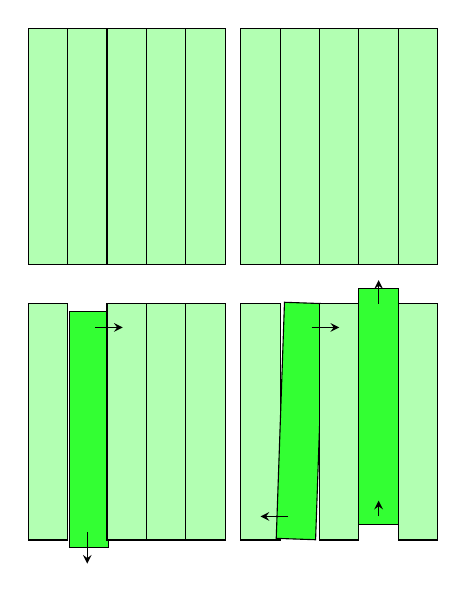
\begin{tikzpicture}
  % this is the ideal detector
  \node[rectangle,
      draw = black,
      % text = ,
      fill = green!30!white,
      minimum width = 0.5cm,
      minimum height = 3cm] (r) at (0,0) {};
  \node[rectangle,
      draw = black,
      % text = ,
      fill = green!80!white,
      minimum width = 0.5cm,
      minimum height = 3cm] (r) at (0.525,-0.1) {};
  \node[rectangle,
      draw = black,
      % text = ,
      fill = green!30!white,
      minimum width = 0.5cm,
      minimum height = 3cm] (r) at (1,0) {};
  \node[rectangle,
      draw = black,
      % text = ,
      fill = green!30!white,
      minimum width = 0.5cm,
      minimum height = 3cm] (r) at (1.5,0) {};
  \node[rectangle,
      draw = black,
      % text = ,
      fill = green!30!white,
      minimum width = 0.5cm,
      minimum height = 3cm] (r) at (2,0) {};

  \node[rectangle,
      draw = black,
      % text = ,
      fill = green!30!white,
      minimum width = 0.5cm,
      minimum height = 3cm] (r) at (2.7,0) {};
  \node[rectangle,
      draw = black,
      % text = ,
      fill = green!80!white,
      rotate around = {-2:(3.2,0)},
      minimum width = 0.5cm,
      minimum height = 3cm] (r) at (3.2,-0.1) {};
  % \draw (2.7,0) -- (5.7,0);
  \node[rectangle,
      draw = black,
      % text = ,
      fill = green!30!white,
      minimum width = 0.5cm,
      minimum height = 3cm] (r) at (3.7,0) {};
  \node[rectangle,
      draw = black,
      % text = ,
      fill = green!80!white,
      minimum width = 0.5cm,
      minimum height = 3cm] (r) at (4.2,0.2) {};
  \node[rectangle,
      draw = black,
      % text = ,
      fill = green!30!white,
      minimum width = 0.5cm,
      minimum height = 3cm] (r) at (4.7,0) {};

% now below it the physical detector
\node[rectangle,
    draw = black,
    % text = ,
    fill = green!30!white,
    minimum width = 0.5cm,
    minimum height = 3cm] (r) at (0,3.5) {};
\node[rectangle,
    draw = black,
    % text = ,
    fill = green!30!white,
    minimum width = 0.5cm,
    minimum height = 3cm] (r) at (0.5,3.5) {};
\node[rectangle,
    draw = black,
    % text = ,
    fill = green!30!white,
    minimum width = 0.5cm,
    minimum height = 3cm] (r) at (1,3.5) {};
\node[rectangle,
    draw = black,
    % text = ,
    fill = green!30!white,
    minimum width = 0.5cm,
    minimum height = 3cm] (r) at (1.5,3.5) {};
\node[rectangle,
    draw = black,
    % text = ,
    fill = green!30!white,
    minimum width = 0.5cm,
    minimum height = 3cm] (r) at (2,3.5) {};

\node[rectangle,
    draw = black,
    % text = ,
    fill = green!30!white,
    minimum width = 0.5cm,
    minimum height = 3cm] (r) at (2.7,3.5) {};
\node[rectangle,
    draw = black,
    % text = ,
    fill = green!30!white,
    minimum width = 0.5cm,
    minimum height = 3cm] (r) at (3.2,3.5) {};
\node[rectangle,
    draw = black,
    % text = ,
    fill = green!30!white,
    minimum width = 0.5cm,
    minimum height = 3cm] (r) at (3.7,3.5) {};
\node[rectangle,
    draw = black,
    % text = ,
    fill = green!30!white,
    minimum width = 0.5cm,
    minimum height = 3cm] (r) at (4.2,3.5) {};
\node[rectangle,
    draw = black,
    % text = ,
    fill = green!30!white,
    minimum width = 0.5cm,
    minimum height = 3cm] (r) at (4.7,3.5) {};

% draw arrows indicating the movement
% x and y translation
\draw [-stealth] (0.6,1.2) -- (0.95,1.2);
\draw [-stealth] (0.5,-1.4) -- (0.5,-1.8);

% rotation
\draw [-stealth] (3.35,1.2) -- (3.7,1.2);
\draw [-stealth] (3.05,-1.2) -- (2.7,-1.2);
% single translation
\draw [-stealth] (4.2,1.5) -- (4.2,1.8);
\draw [-stealth] (4.2,-1.2) -- (4.2,-1);

\end{tikzpicture}

    \end{column}
    \begin{column}[c]{0.48\textwidth}
      \begin{itemize}
        \item $\bullet$\, top: ideal detector, bottom: physical detector
        \item $\bullet$\, Surveys are used to find the rotation and position of each detector component
        \item $\bullet$\, Are used as starting positions for software alignment
        \item $\bullet$\, Building tracks accurately requires positions in reconstruction to be as similar as possible to real positions
      \end{itemize}
    \end{column}
  \end{columns}
\end{frame}

\begin{frame}\frametitle{Alignment: track fits with the Kalman Filter}
  \begin{columns}
    \begin{column}[c]{0.4\textwidth}
      \begin{figure}
        \centering
        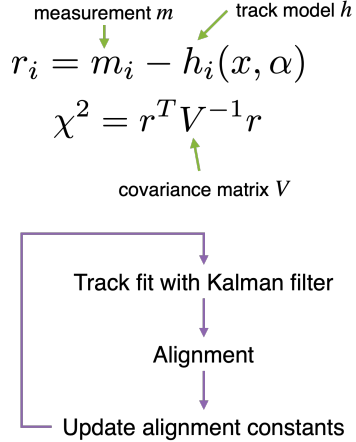
\includegraphics[width=0.72\textwidth]{logos/kalman.png}
        % \caption{Alignment with Kalman Filter.}
      \end{figure}
    \end{column}
    \begin{column}[c]{0.55\textwidth}
      \begin{itemize}
        \item $\bullet$\, Use survey information as starting point
        \item $\bullet$\, aligning the detector by minimizing the residuals of the track hits
        \item $\bullet$\, basically a $\chi^2$ minimization problem with alignment parameters $\alpha$
        \item $\bullet$\, Why Kalman Filter?
        \begin{itemize}
          \item $\bullet$\, easily models material interactions as well as multiple scattering
        \end{itemize}
        \item $\bullet$\, propagation of nodes, minimization, smooth error sizes by back propagation
      \end{itemize}
    \end{column}
  \end{columns}
\end{frame}

\begin{frame}\frametitle{Importance of alignments}
  \begin{itemize}
    \item $\bullet$\, Alignment is part of the LHCb trigger system
    \item $\bullet$\, Physics performance tied to alignment performance
    \item $\bullet$\, with optimal alignment:
    \begin{itemize}
      \item $\bullet$\, \to\, remove systematic biases for asymmetry measurements
      \item $\bullet$\, best possible mass resolution
    \end{itemize}
  \end{itemize}
  \begin{figure}
      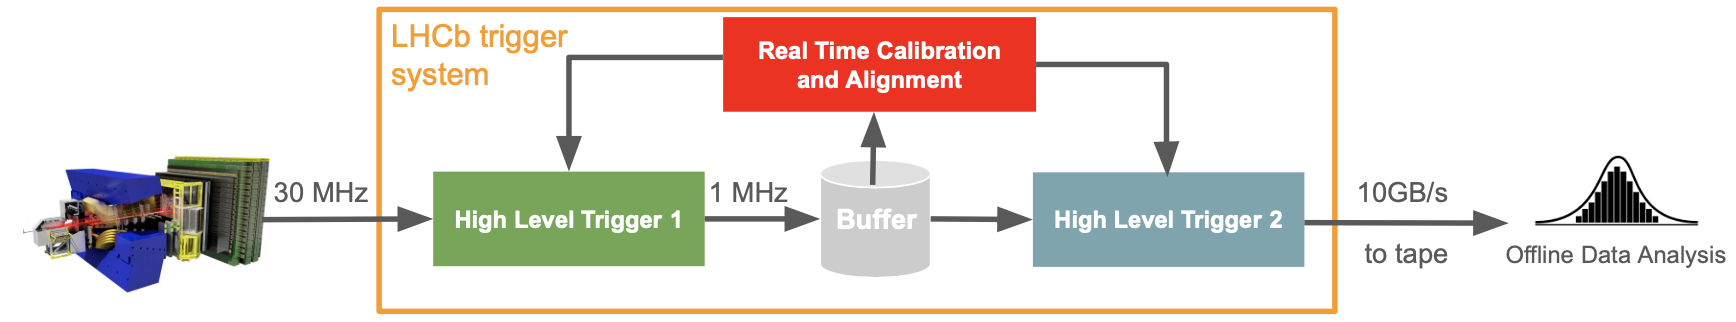
\includegraphics[width=0.9\textwidth]{logos/dataflow.png}%
    % \caption{Hits on tracks in x-direction with run 256145 data on 20000 ents using 9 minimum hits against 11 minimum hits.}
  \end{figure}
\end{frame}

\begin{frame}\frametitle{LHCb upgraded with the SciFi}
  \begin{columns}
    \begin{column}[c]{0.48\textwidth}
      \begin{figure}
        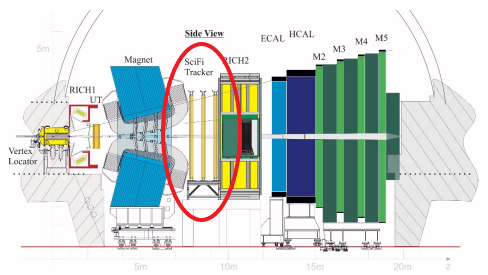
\includegraphics[width=\textwidth]{logos/upgrade_lhcb.png}
        % \caption{Visualization of the SciFi tracking stations.}
      \end{figure}
    \end{column}
    \begin{column}{0.48\textwidth}
      \begin{itemize}
        \item $\bullet$\, Consists of 3 stations: T1, T2, T3
        \item $\bullet$\, 4 layers per station: X1, U, V, X2
      	\item $\bullet$\, replaces former IT and OT to cope with the increased instantaneous luminosity
	      \item $\bullet$\, crucial part of tracking system
      \end{itemize}
      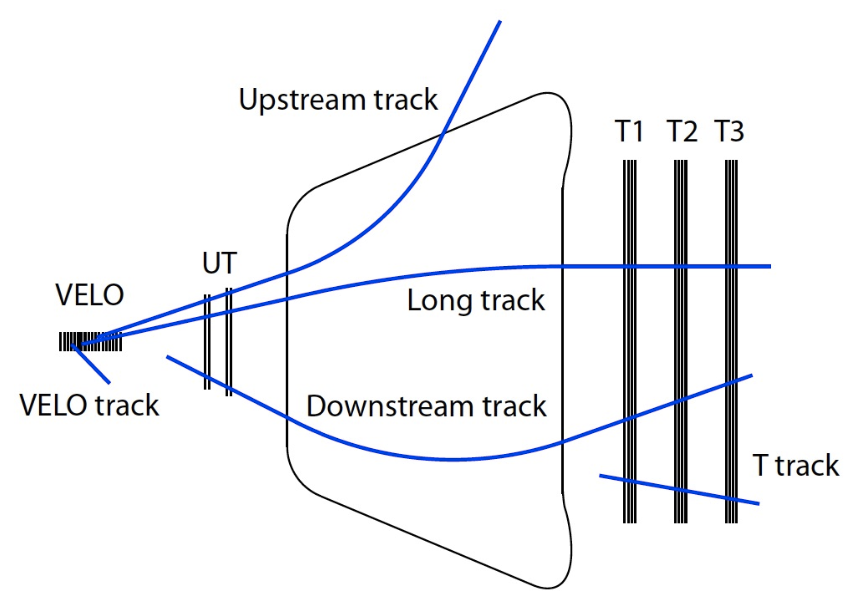
\includegraphics[width=0.5\textwidth]{track.png}
    \end{column}
  \end{columns}
\end{frame}

\begin{frame}\frametitle{The Scintillating Fibre Tracker}
  \begin{columns}
    \begin{column}[c]{0.48\textwidth}
      \begin{figure}
        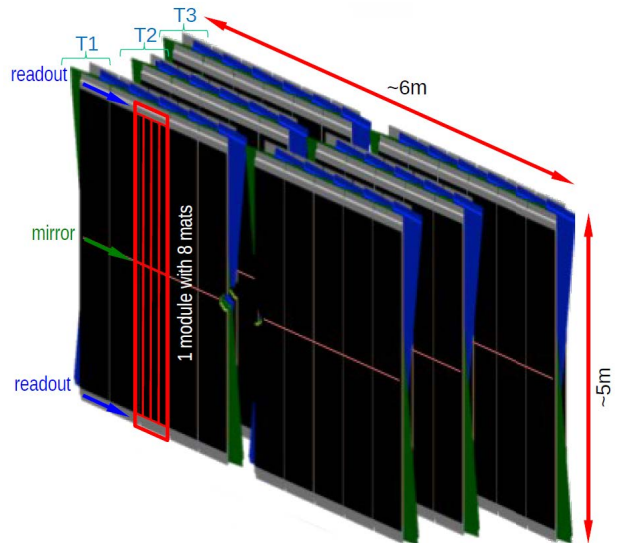
\includegraphics[width=0.9\textwidth]{logos/scifi.png}
        % \caption{Visualization of the SciFi tracking stations.}
      \end{figure}
    \end{column}
    \begin{column}{0.48\textwidth}
      \begin{itemize}
        \item $\bullet$\, Front two stations have 5 modules per side
        \item $\bullet$\, Back station has 6 modules on each side
        \item $\bullet$\, U, V layers have a $\mp 5 \deg$ stereo angle respectively
        \item $\bullet$\, \to\, used for determining y-position of tracks by comparing hitposition at different angles
      \end{itemize}
    \end{column}
  \end{columns}
\end{frame}

\begin{frame}\frametitle{SciFi terminology}
  layers are divided into two halves commonly labeled as A-side and C-side
  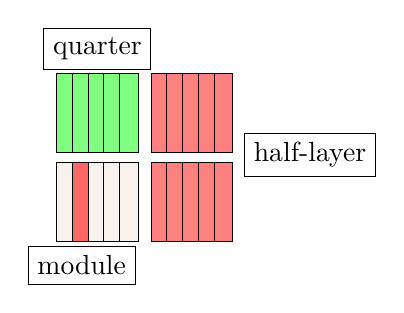
\begin{tikzpicture}
% first quarter
  \node[rectangle,
      draw = black,
      % text = ,
      fill = brown!10!white,
      minimum width = 0.2cm,
      minimum height = 1cm] (r) at (0,0) {};

  \node[rectangle,
      draw = black,
      % text = half-module,
      fill = red!60!white,
      minimum width = 0.2cm,
      minimum height = 1cm] (r) at (0.2,0) {};

  \node[rectangle,
      draw = black,
      % text = ,
      fill = brown!10!white,
      minimum width = 0.2cm,
      minimum height = 1cm] (r) at (0.4,0) {};

  \node[rectangle,
      draw = black,
      % text = ,
      fill = brown!10!white,
      minimum width = 0.2cm,
      minimum height = 1cm] (r) at (0.6,0) {};

  \node[rectangle,
      draw = black,
      % text = ,
      fill = brown!10!white,
      minimum width = 0.2cm,
      minimum height = 1cm] (r) at (0.8,0) {};

% second quarter
\node[rectangle,
    draw = black,
    % text = ,
    fill = red!50!white,
    minimum width = 0.2cm,
    minimum height = 1cm] (r) at (1.2,0) {};

\node[rectangle,
    draw = black,
    % text = ,
    fill = red!50!white,
    minimum width = 0.2cm,
    minimum height = 1cm] (r) at (1.4,0) {};

\node[rectangle,
    draw = black,
    % text = ,
    fill = red!50!white,
    minimum width = 0.2cm,
    minimum height = 1cm] (r) at (1.6,0) {};

\node[rectangle,
    draw = black,
    % text = ,
    fill = red!50!white,
    minimum width = 0.2cm,
    minimum height = 1cm] (r) at (1.8,0) {};

\node[rectangle,
    draw = black,
    % text = ,
    fill = red!50!white,
    minimum width = 0.2cm,
    minimum height = 1cm] (r) at (2,0) {};

% third quarter
\node[rectangle,
    draw = black,
    % text = ,
    fill = green!50!white,
    minimum width = 0.2cm,
    minimum height = 1cm] (r) at (0,1.13) {};

\node[rectangle,
    draw = black,
    % text = quarter,
    fill = green!50!white,
    minimum width = 0.2cm,
    minimum height = 1cm] (r) at (0.2,1.13) {};

\node[rectangle,
    draw = black,
    % text = ,
    fill = green!50!white,
    minimum width = 0.2cm,
    minimum height = 1cm] (r) at (0.4,1.13) {};

\node[rectangle,
    draw = black,
    % text = ,
    fill = green!50!white,
    minimum width = 0.2cm,
    minimum height = 1cm] (r) at (0.6,1.13) {};

\node[rectangle,
    draw = black,
    % text = ,
    fill = green!50!white,
    minimum width = 0.2cm,
    minimum height = 1cm] (r) at (0.8,1.13) {};

% fourth quarter
\node[rectangle,
    draw = black,
    % text = ,
    fill = red!50!white,
    minimum width = 0.2cm,
    minimum height = 1cm] (r) at (1.2,1.13) {};

\node[rectangle,
    draw = black,
    % text = ,
    fill = red!50!white,
    minimum width = 0.2cm,
    minimum height = 1cm] (r) at (1.4,1.13) {};

\node[rectangle,
    draw = black,
    % text = ,
    fill = red!50!white,
    minimum width = 0.2cm,
    minimum height = 1cm] (r) at (1.6,1.13) {};

\node[rectangle,
    draw = black,
    % text = ,
    fill = red!50!white,
    minimum width = 0.2cm,
    minimum height = 1cm] (r) at (1.8,1.13) {};

\node[rectangle,
    draw = black,
    % text = ,
    fill = red!50!white,
    minimum width = 0.2cm,
    minimum height = 1cm] (r) at (2,1.13) {};

\node[draw] at (0.4, 1.95) {quarter};
\node[draw] at (0.2, -0.8) {module};
\node[draw] at (3.1, 0.6) {half-layer};

\end{tikzpicture}

\end{frame}

\begin{frame}\frametitle{The survey: what is it and the different types}
  \begin{columns}
    \begin{column}[c]{0.48\textwidth}
      $\bullet$\, measure distance of some points on the detector with a laser
      \begin{figure}
        \centering
        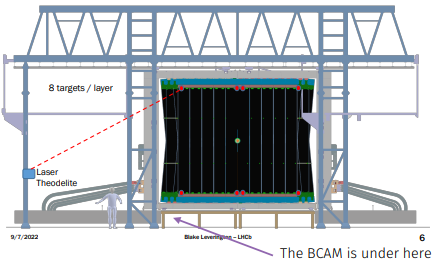
\includegraphics[width=\textwidth]{logos/survey.png}
        % \caption{}
      \end{figure}
    \end{column}
    \begin{column}[c]{0.48\textwidth}
      \begin{itemize}
        \item $\bullet$\, 2022: photogrammetry (assembly hall) \to\, not quite perfect
        \item $\bullet$\, 2023: cavern
        \item $\bullet$\, compare survey to simulation
        \item $\bullet$\, layer survey: coarse, survey layer positions
        \item $\bullet$\, module survey: keep track of each module
      \end{itemize}
    \end{column}
  \end{columns}
\end{frame}

\begin{frame}\frametitle{Alignment versions in use}
  \begin{columns}
    \begin{column}[c]{0.4\textwidth}
      \centering
      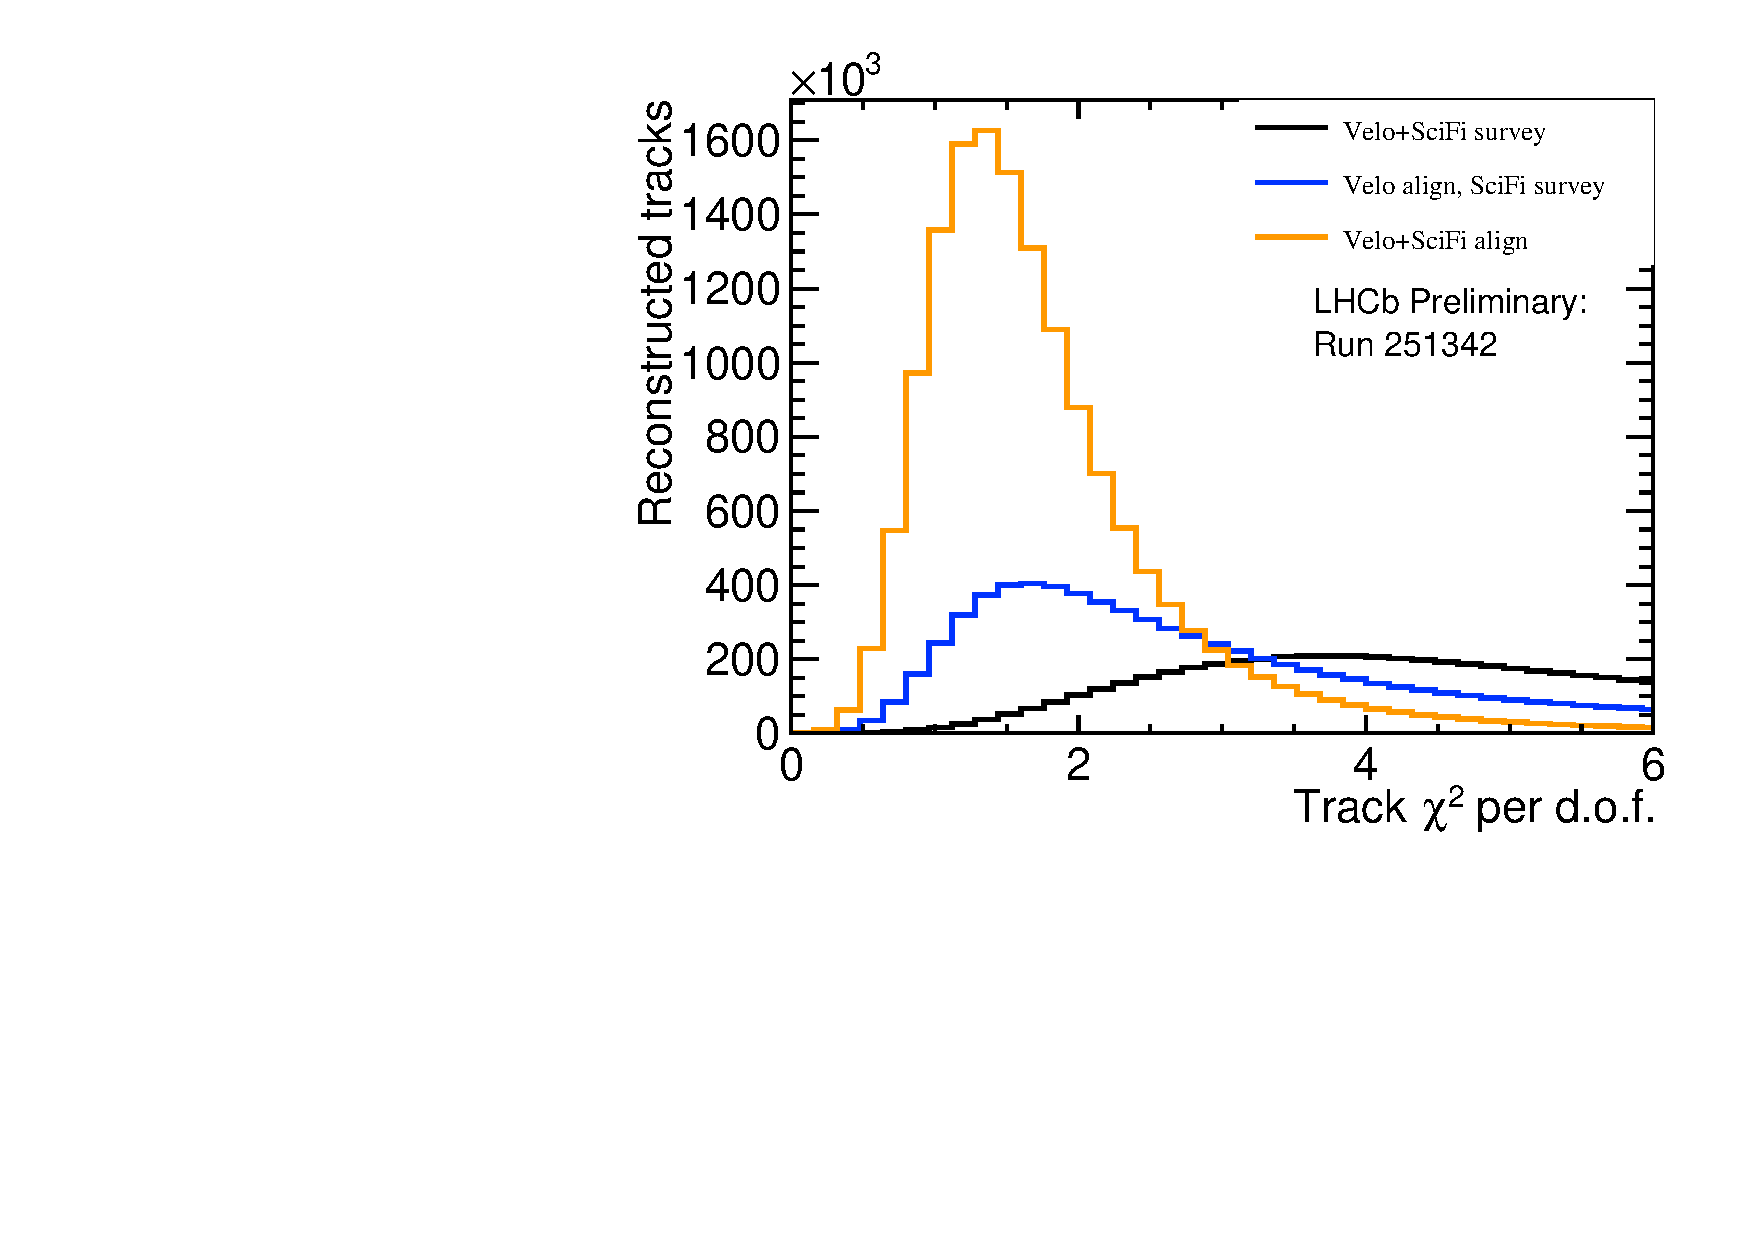
\includegraphics[width=\textwidth]{logos/LHCb-FIGURE-2022-018/Run251342Preliminary_BestLong_chi2_per_ndof.pdf}
    \end{column}
    \begin{column}[c]{0.3\textwidth}
      \begin{itemize}
        \item $\bullet$\, V1: First ever alignments after upgrade
      	\item $\bullet$\, Using first data sets
        \item $\bullet$\, Starting configyartion: long modules, Tx Rz
      \end{itemize}
    \end{column}
    \begin{column}[c]{0.3\textwidth}
      \begin{itemize}
        \item $\bullet$\, V2: Imroved configuaration from V1 %(hard work from detector experts)
        \item $\bullet$\, half modules, Tx Rz, new time alignment
      \end{itemize}
    \end{column}
  \end{columns}
\end{frame}

\begin{frame}\frametitle{Hit distribution per quarter in V1 and V2 alignment}
  \begin{itemize}
    \item $\bullet$\, A-side improved a lot in V2, losing some performance on C-side
    \item $\bullet$\, Performance discrepancies \to quarter analysis
    \item $\bullet$\, $\chi2$ per quarter \to alignment performance per detector part
  \end{itemize}
  \begin{mybox}{green}{}
    \begin{itemize}
      \item $\bullet$\, Scan quarters individually; find issues faster
    \end{itemize}
  \end{mybox}
  \begin{figure}
      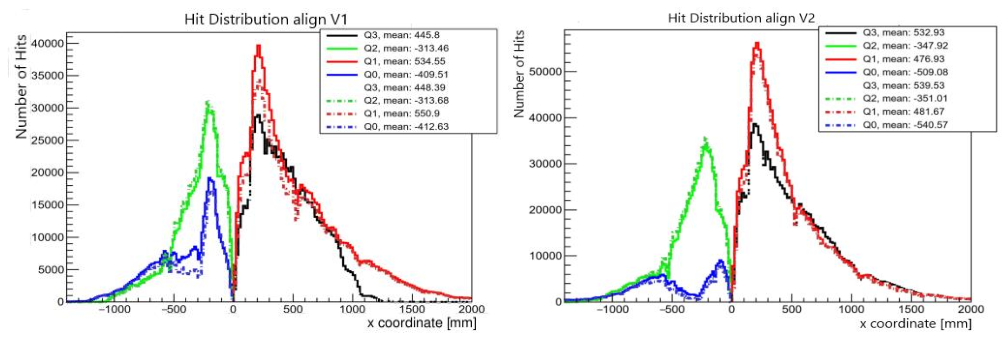
\includegraphics[width=0.8\textwidth]{logos/v1_v2.png}%
      % 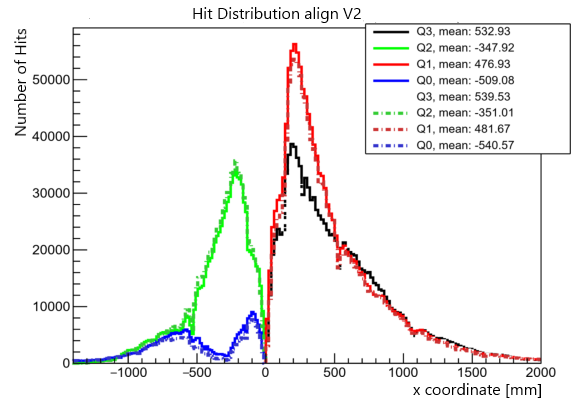
\includegraphics[width=0.45\textwidth]{logos/hit_dist_v2.png}%
  \end{figure}
\end{frame}

\begin{frame}\frametitle{Track hits comparison of V2 and simulation}
\begin{mybox}{green}{}
  \begin{itemize}
    \item $\bullet$\, Simulation: hits on \textbf{reconstructed} tracks fill whole detector
    \item $\bullet$\, data: filling tracks into A-side \to\, good!
  \end{itemize}
\end{mybox}
\begin{mybox}{orange}{}
  \begin{itemize}
    \item \to\, scan C-side quarters for possible issues in distinct layers
  \end{itemize}
\end{mybox}
  \begin{columns}
    \begin{column}[c]{0.48\textwidth}
      \begin{figure}
        \centering
        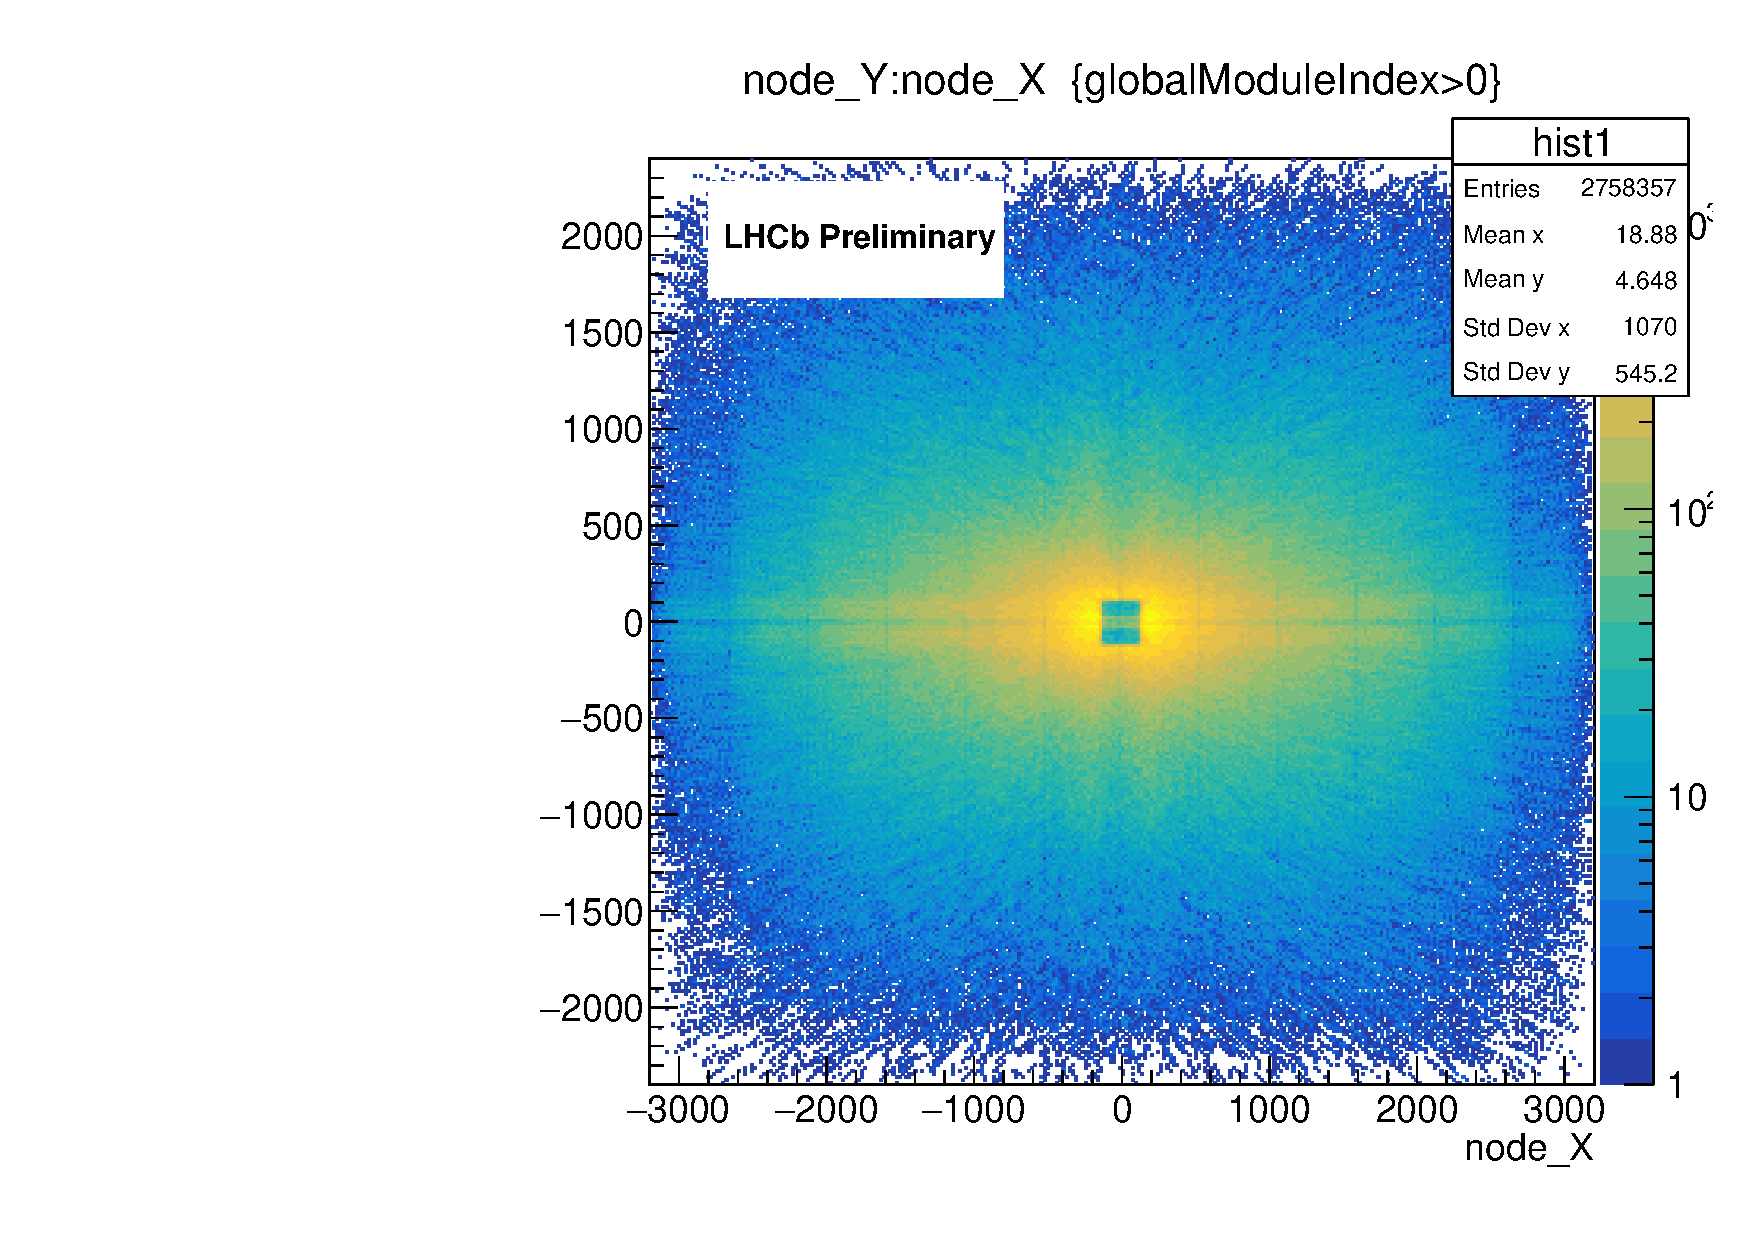
\includegraphics[width=0.6\textwidth]{logos/nodeXY_MC.pdf}%
      \end{figure}
    \end{column}
    \begin{column}[c]{0.48\textwidth}
      \begin{figure}
        \centering
        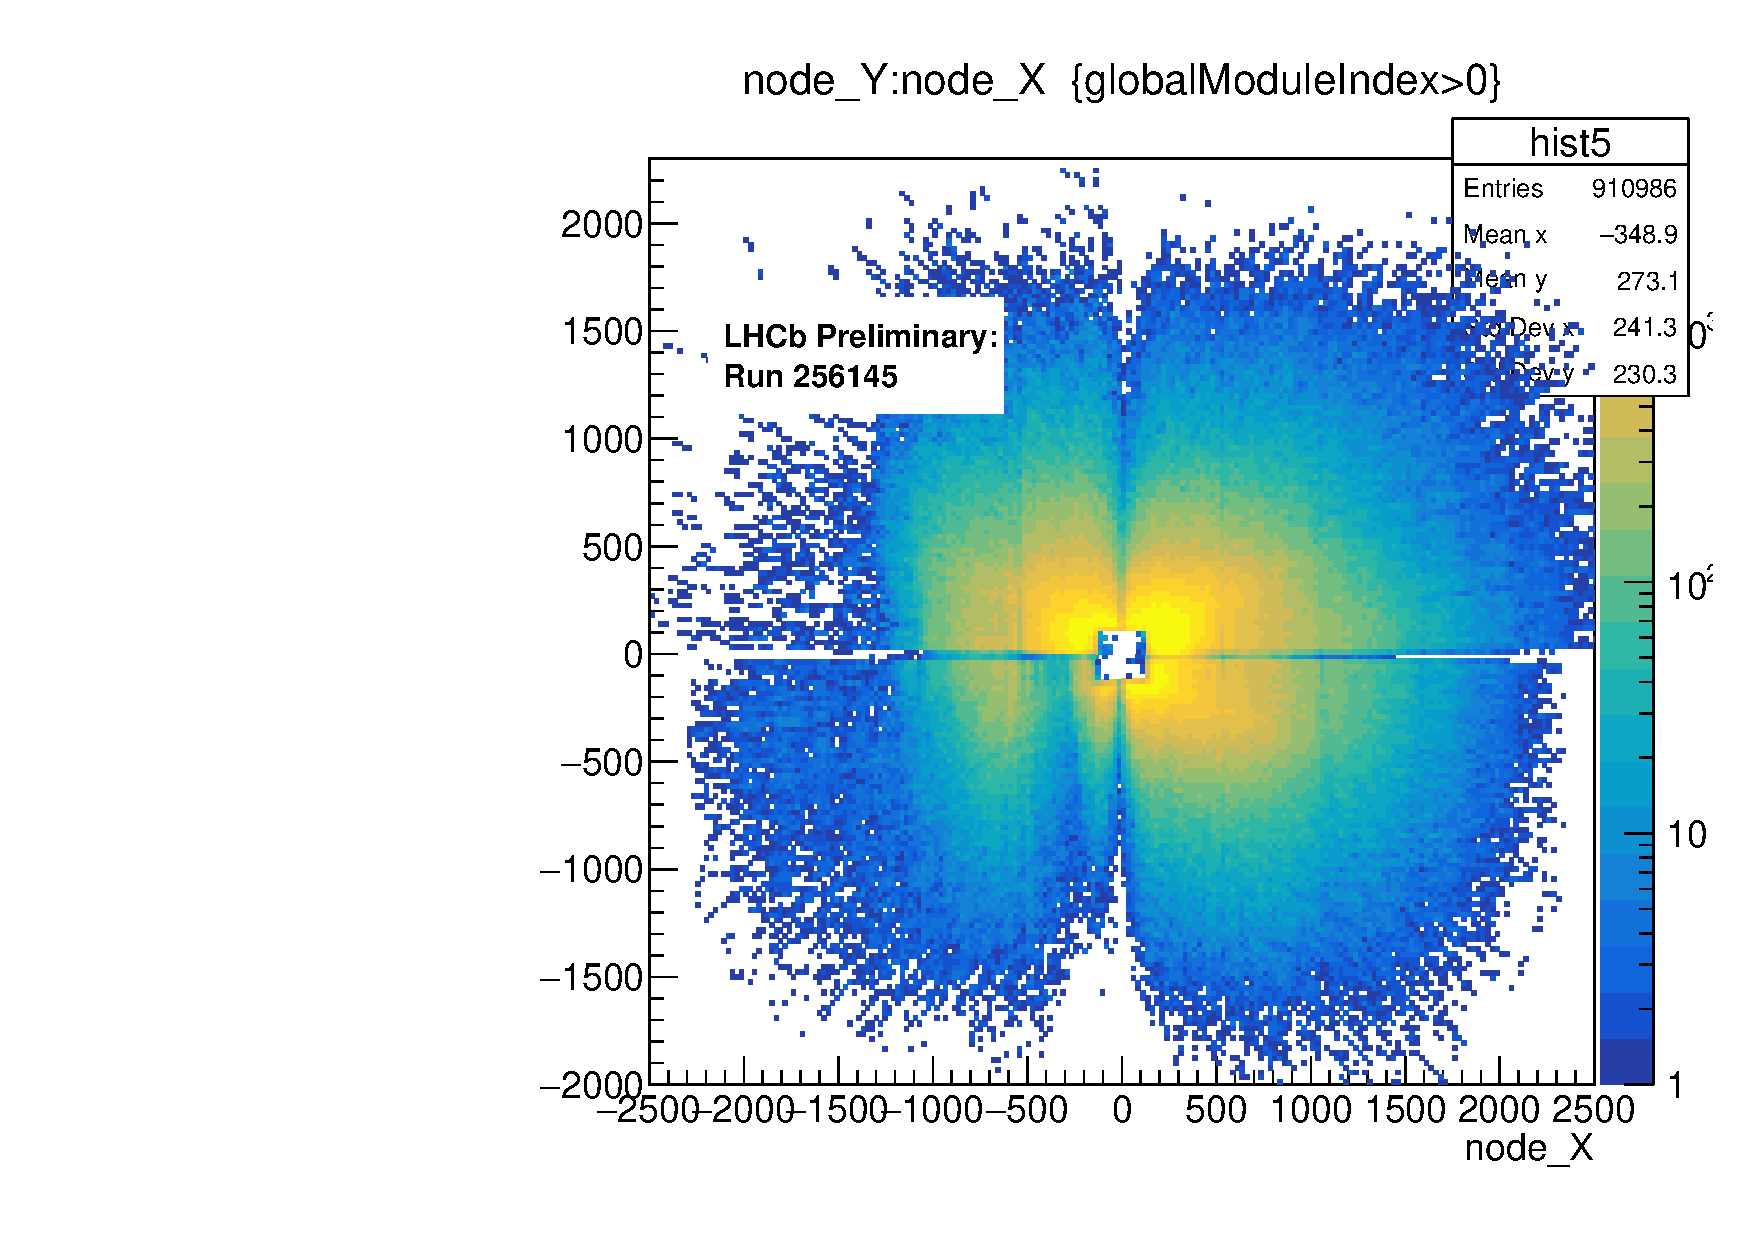
\includegraphics[width=0.6\textwidth]{tuples_out/combining_2D_nodeXY_v2.pdf}%
      \end{figure}
    \end{column}
  \end{columns}
\end{frame}

\begin{frame}\frametitle{Improved Q0 positions in T2X2 layer with V2 alignment}
  \begin{itemize}
    \item $\bullet$\, manual comparison of striking features in problematic layer
    % \item $\bullet$\, positions: translations relative to the nominal position for each module
    \item $\bullet$\, Q0 too far out of alignment \to less hits
    \item $\bullet$\, Manual scans + looser tracking config \to Alignment V3
  \end{itemize}
  \begin{figure}
    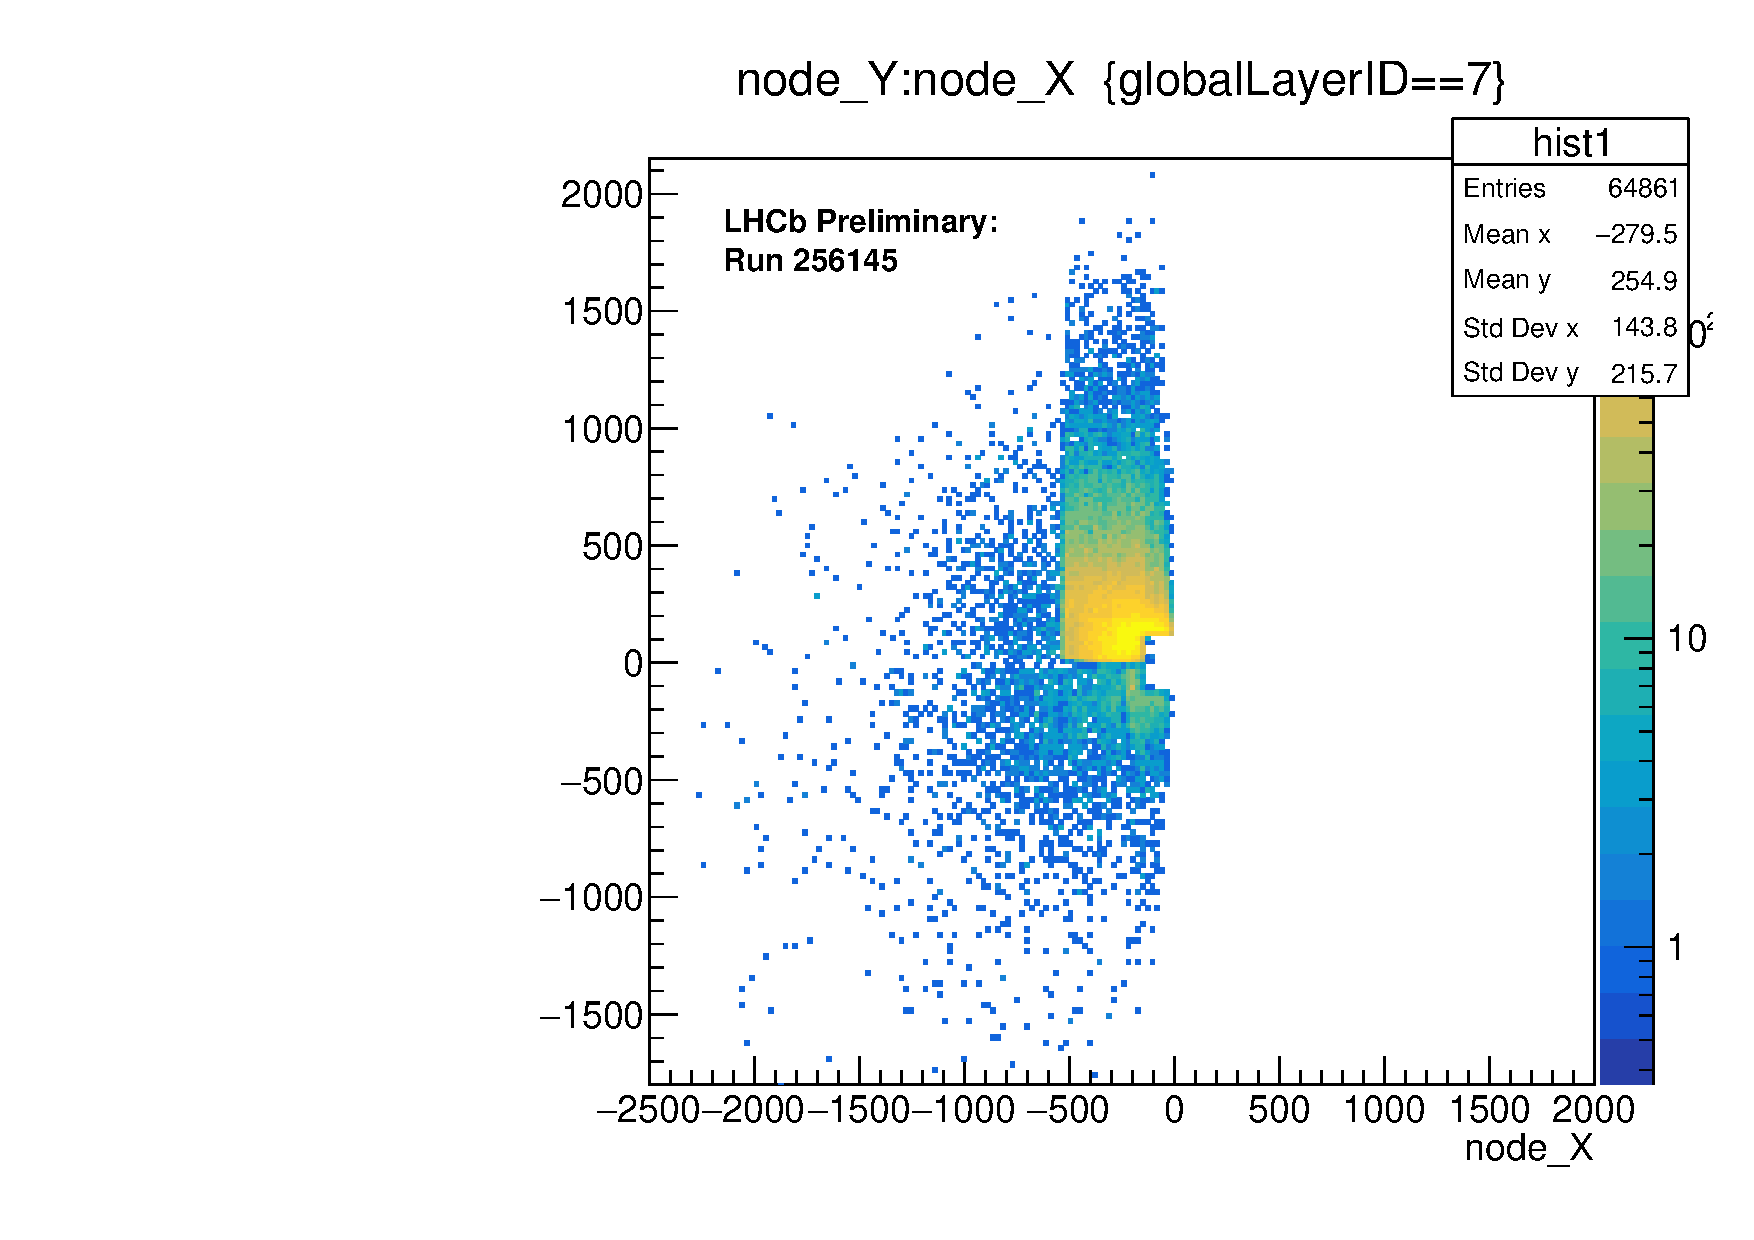
\includegraphics[width=0.26\textwidth]{logos/2D_nodeXY_v2_7_left.pdf}%
    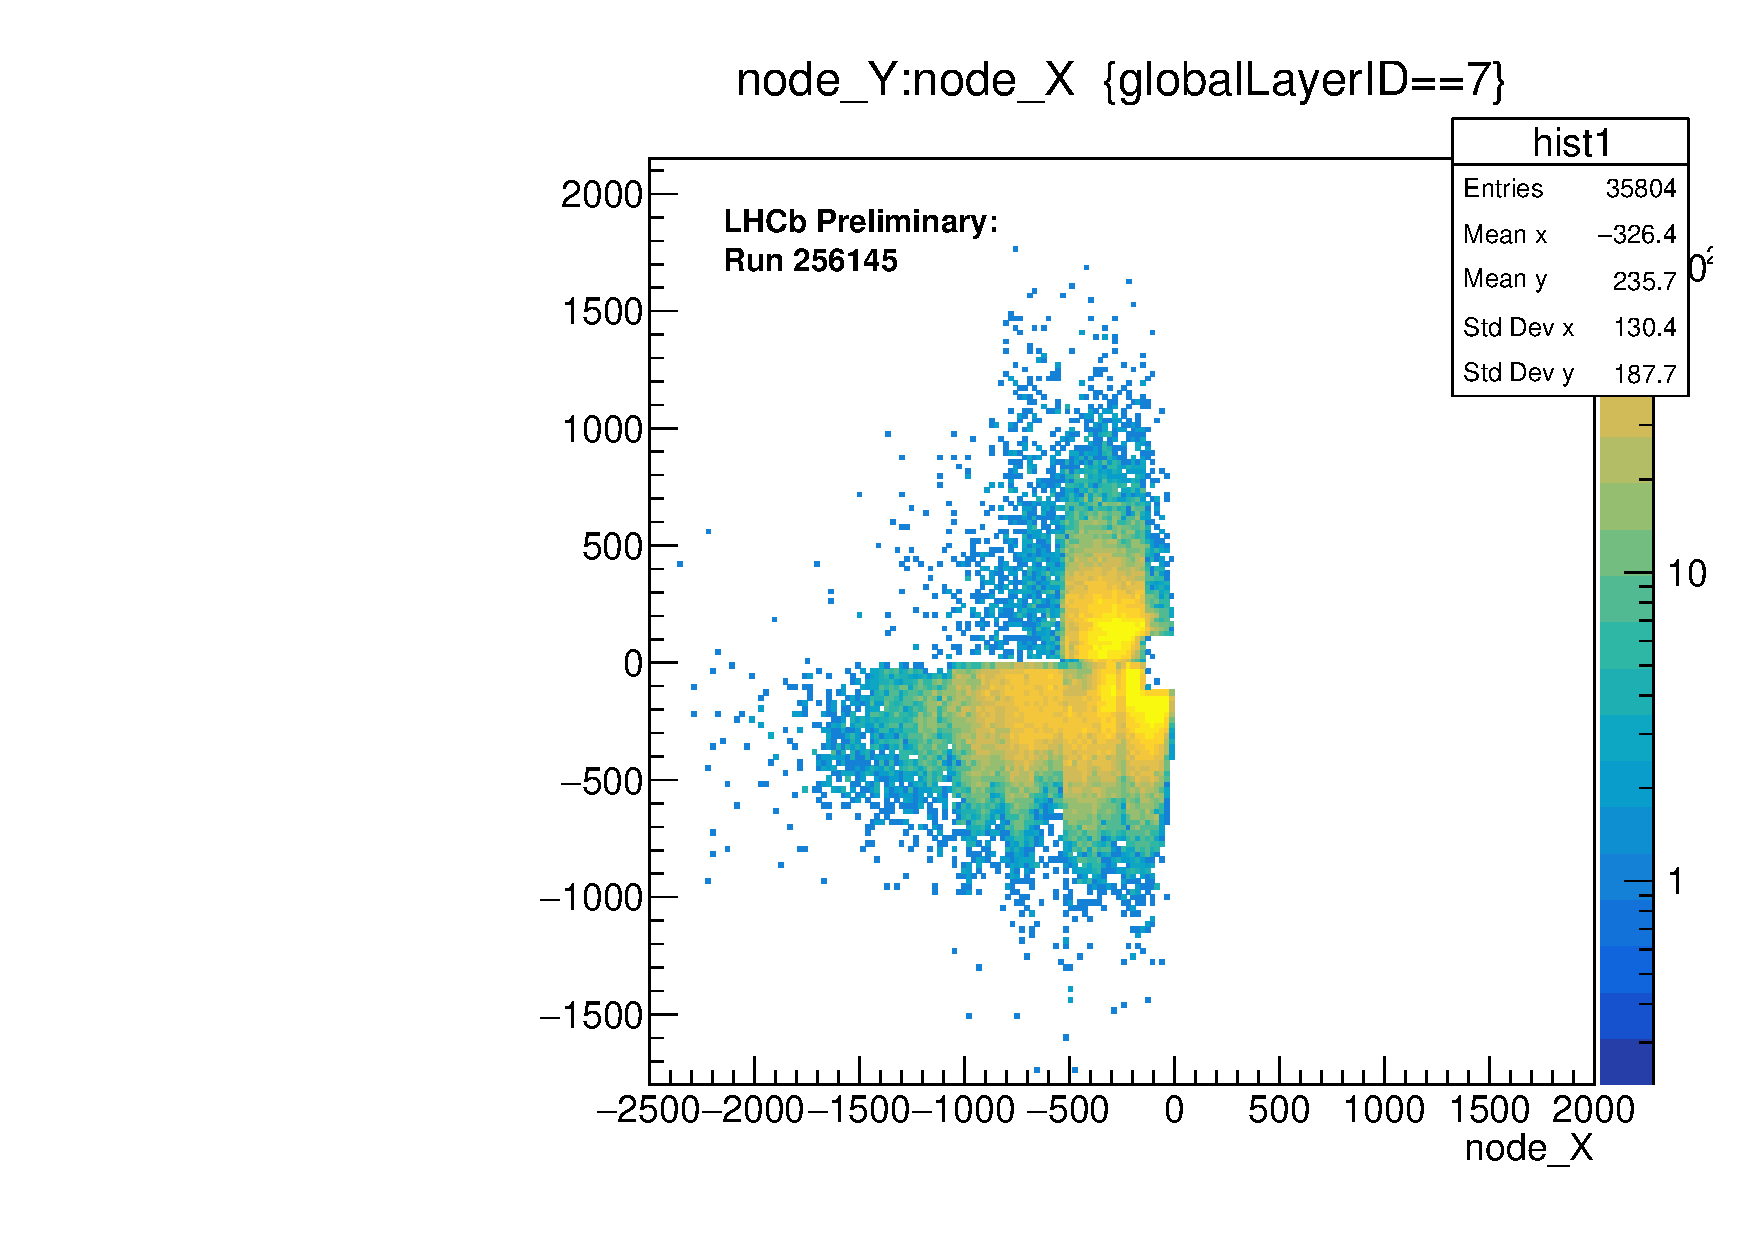
\includegraphics[width=0.26\textwidth]{logos/2D_nodeXY_quartermean_7_left.pdf}%
    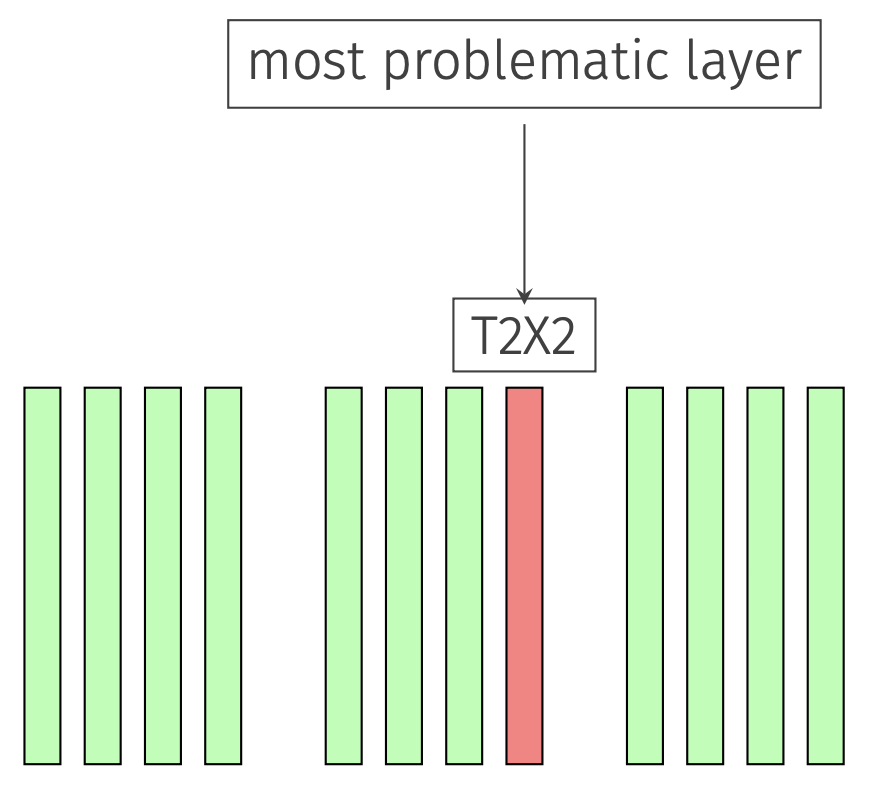
\includegraphics[width=0.26\textwidth]{problem_layer.png}%
  \end{figure}
\end{frame}

\begin{frame}\frametitle{Stability tests on 2022 data}
  \begin{columns}
    \begin{column}[c]{0.4\textwidth}
      \begin{itemize}
        \setlength\itemsep{1em}
        \item $\bullet$\, \textbf{How much does the SciFi move between runs?}
        \item $\bullet$\, \textbf{Does the magnet polarity impact playa role in the alignment?}
      \end{itemize}
    \end{column}
    \begin{column}[c]{0.6\textwidth}
      \begin{itemize}
        \item $\bullet$\, Run an alignment for each of the runs on the list
        \item $\bullet$\, Sort the runs in ascending run number
        \item $\bullet$\, Compare the difference in module position for each run to the next
        \item $\bullet$\, Where are the modules in the local frame in all runs?
      \end{itemize}
    \end{column}
  \end{columns}
\end{frame}

\begin{frame}\frametitle{Module Positions in local half module frame}
  \begin{columns}
    \begin{column}[c]{0.35\textwidth}
      \begin{itemize}
        \setlength\itemsep{0em}
        \item $\bullet$\, Runs 255949 + 256030 problematic \to issues known!
        \item $\bullet$\, Optimal fine timing implemented in 256145 (afterwards)
        \item $\bullet$\, Both magnet polarities comparable results
      \end{itemize}
    \end{column}
    \begin{column}[c]{0.65\textwidth}
      \begin{figure}
        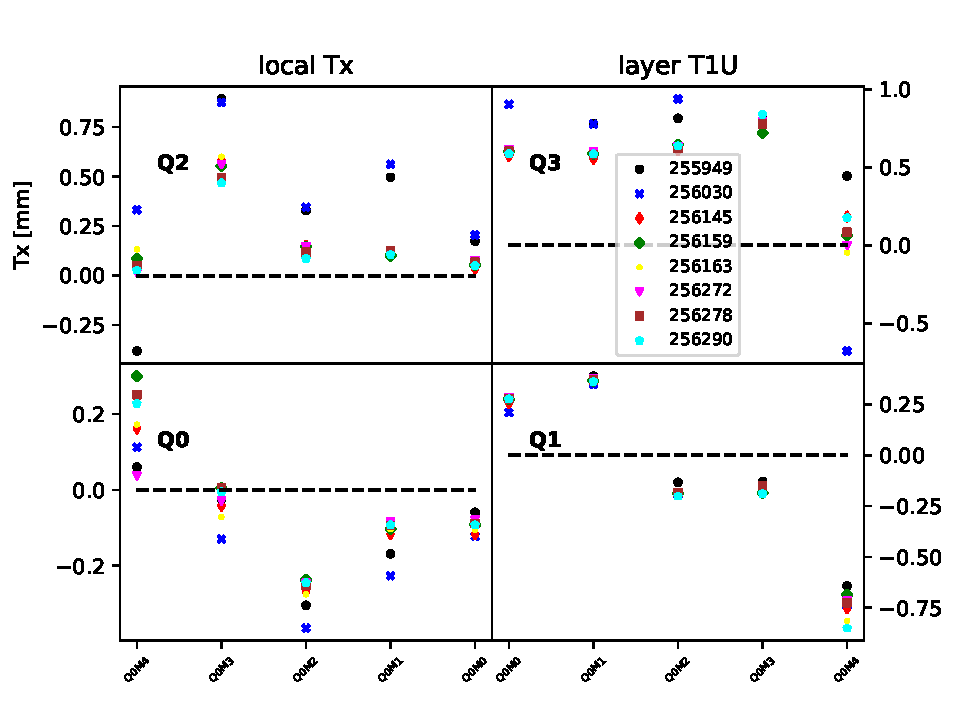
\includegraphics[width=0.9\textwidth]{plots/plain_data/raw_data_T1U_Tx.pdf}
      \end{figure}
    \end{column}
  \end{columns}
\end{frame}

\begin{frame}\frametitle{Reduced dataset: removed pre timing update runs}
  \begin{columns}
    \begin{column}[c]{0.48\textwidth}
      \begin{itemize}
        \item $\bullet$\, comparison of module positions of 2 runs each
        % \item $\bullet$\, Without the fine timing changes the largest movement is at max around $400 \mu m$ at most outer modules
        \item $\bullet$\, Outer modules \to low statistics \to difficult for the alignment \to large movement
        \item $\bullet$\, Inner modules: movement around $150 \mu m$ allowed
      \end{itemize}
    \end{column}
      \begin{column}[c]{0.48\textwidth}
        \begin{figure}
          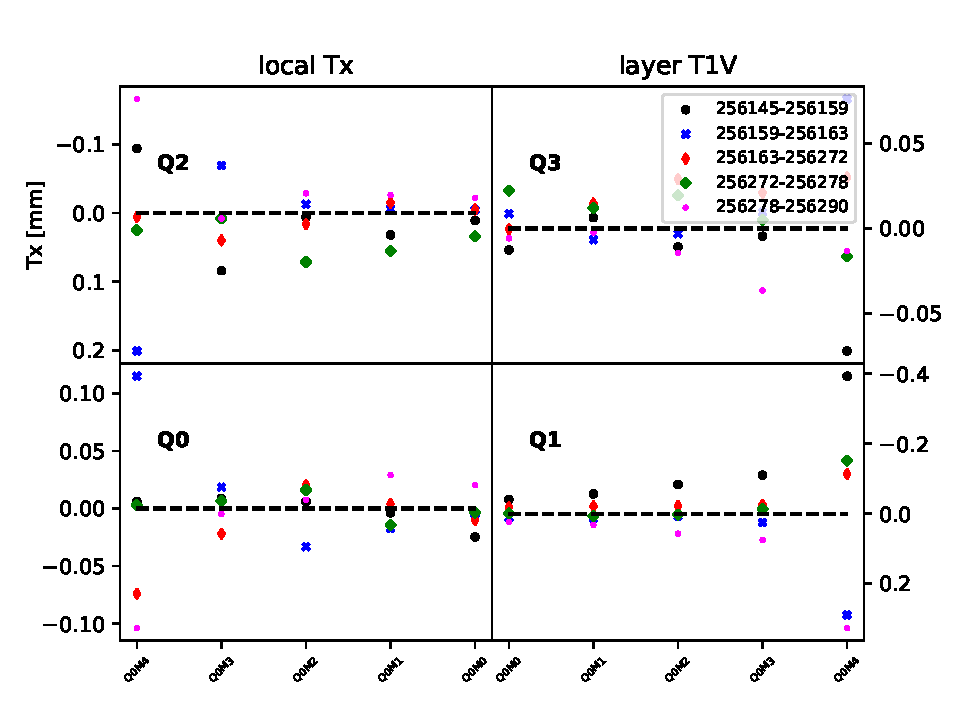
\includegraphics[width=\textwidth]{plots/stability_plots/diff_reduced_Tx_T1V_Tx.pdf}
        \end{figure}
      \end{column}
  \end{columns}
\end{frame}

\begin{frame}\frametitle{stability tests: Conclusion}
  \begin{columns}
    \begin{column}[c]{\textwidth}
      \begin{itemize}
        \item $\bullet$\, Timing changes have big impact on module alignment
        \item $\bullet$\, The change in module position from run to run is at maximum $150 \mu m$ for the modules M0 \to M3 in Tx
        \item \to only if there are no big changes between runs
        \item $\bullet$\, M4 moves at max $400 \mu m$ in this case
        \item $\bullet$\, there is no visible difference between magUp and magDown polarity
        \item $\bullet$\, With good SciFi timing, variation of 200 $\mu m$ expected.
        \item $\bullet$\, A possible choice of an automatic update would be if variations of > 200 $\mu m$ occur.
      \end{itemize}
    \end{column}
  \end{columns}
\end{frame}

% \begin{frame}\frametitle{Joints constraints for SciFi module alignment}
%   \begin{columns}
%     \begin{column}[c]{0.6\textwidth}
%       \begin{itemize}
%         \setlength\itemsep{0em}
%         \item $\bullet$\, Long SciFi modules: slight "banana shape"
%         \item $\bullet$\, Half modules + joints reproduce the real shape
%         \item $\bullet$\, Joints are implemented in the alignment by using a survey constraint (\href{https://gitlab.cern.ch/lhcb/Alignment/-/merge_requests/368}{MR!368})
%         \item $\bullet$\, it constrains parameters of 2 alignables A and B to each other with $\chi^2 = \left( p_A - p_B \right)^T V^{-1} \left( p_A - p_B \right)$
%         \item $\bullet$\, $p_A,p_B$: set of parameters for half modules
%         \item $\bullet$\, use common frame (local half modules)
%         \item $\bullet$\, Uncertainties taken from diagonal covariance matrix \to how realistic? \to tuning needed
%         \item $\bullet$\, No existing survey available for joints; tuning needed to control their $\chi^2$
%       \end{itemize}
%     \end{column}
%       \begin{column}[c]{0.4\textwidth}
%         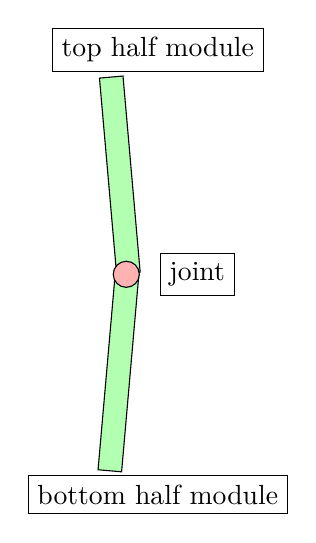
\begin{tikzpicture}
    \node[rectangle, 
    draw = black, 
    fill = green!30!white, 
    minimum width = 0.3cm, 
    minimum height = 2.5cm,
    rotate around = {-5:(0,0)}] at (0,0) {};
    \node[rectangle, 
    draw = black, 
    fill = green!30!white, 
    minimum width = 0.3cm, 
    minimum height = 2.5cm,
    rotate around = {5:(0,2.5)}] at (-0.2,2.5) {};
    \node[circle, 
    draw = black, 
    fill = red!30!white, 
    minimum width = 0.01cm] at (0.1,1.25) {};

    \node[draw, align=left] at (0.5, 4.1) {top half module};
    \node[draw, align=left] at (1, 1.25) {joint};
    \node[draw, align=left] at (0.5, -1.55) {bottom half module};
\end{tikzpicture}
%       \end{column}
%   \end{columns}
% \end{frame}

% \begin{frame}\frametitle{Tuning procedure}
%   \begin{columns}
%     \begin{column}[c]{0.48\textwidth}
%       \begin{itemize}
%         \setlength\itemsep{0em}
%         \item $\bullet$\, Instead of one $\chi^2$ \to look at $\chi^2$ for joint parameters (Tx, Ty, Tz, Rx, Ry, Rz)
%         \item $\bullet$\, Tune Uncertainties by running an alignment for each change to the respective parameter uncertainty until roughly $\chi^2 / \text{DoF} = 1$
%         \item $\bullet$\, make sure not to run into local minimum
%       \end{itemize}
%     \end{column}
%       \begin{column}[c]{0.48\textwidth}
%         \begin{itemize}
%           \item $\bullet$\, Procedure evaluated with 2023 data (run 269045, warm SciFi) and master from conditions database
%           \item $\bullet$\, Using the alignment master
%         \end{itemize}
%         \begin{figure}
%           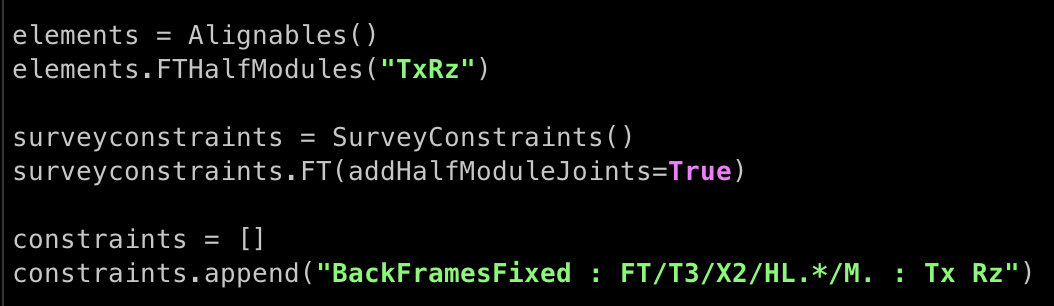
\includegraphics[width=\textwidth]{plots/config_joint_constraint.png}
%         \end{figure}
%       \end{column}
%   \end{columns}
% \end{frame}

% \begin{frame}\frametitle{Tuning of uncertainty: Tx}
%   \begin{columns}
%     \begin{column}[c]{0.48\textwidth}
%       Initial errors:
%       \begin{itemize}
%         \setlength\itemsep{0em}
%         \item $\bullet$\, Tx,Ty,Tz [$\mu m$]: 1 1 1
%         \item $\bullet$\, Rx,Ry,Rz [$\text{mrad}$]: 0.2 0.2 0.2
%         \item $\bullet$\, Vary Tx uncertainty (starting at 1 $\mu m$) \to run alignment \to calculate $\chi^2/\text{DoF}$ values, keep other parameters at nominal!
%         \item \to $\text{Tx}= 1\mu m$ has $\chi^2 \approx 13$, perform a scan in a range of uncertainties to find the intersection $\chi^2/\text{DoF} = 1$ (black line)
%       \end{itemize}
%     \end{column}
%       \begin{column}[c]{0.48\textwidth}
%         intersection: $0.22 \mu m$ (fit), $0.3 \mu m$ (measurement)
%         \begin{figure}
%           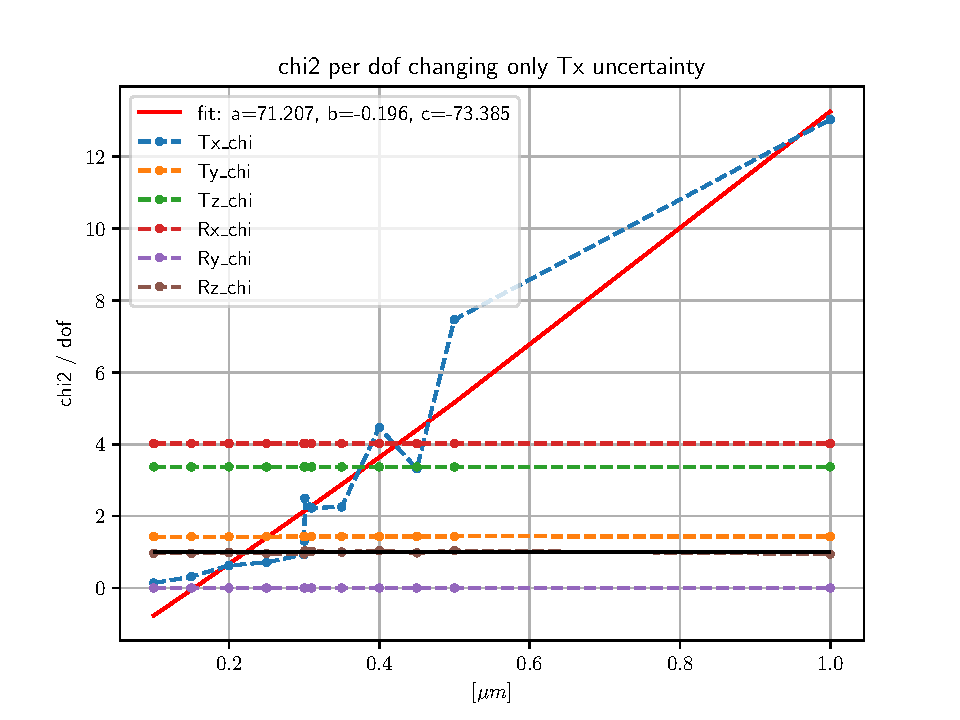
\includegraphics[width=\textwidth]{plots/retest/only_Tx_full_fit.pdf}
%         \end{figure}
%       \end{column}
%     \end{columns}
%   \end{frame}

% \begin{frame}\frametitle{Tuning of uncertainty: Rz}
%   \begin{columns}
%     \begin{column}[c]{0.48\textwidth}
%       Initial errors:
%       \begin{itemize}
%         \setlength\itemsep{0em}
%         \item $\bullet$\, In the last step Rz was tuned
%         \item $\bullet$\, intersection at 0.2 mrad was already correctly set from nominal
%         \item $\bullet$\, All parameters show good behaviour at chosen uncertainty
%         \item $\bullet$\, final tunded uncertainties [$\mu m$, mrad]: 0.3 1.2 1.9 0.4 0.00000044 0.2
%         % \item $\bullet$\, \textbf{make a slide with the tests for loose particle selection}
%       \end{itemize}
%     \end{column}
%       \begin{column}[c]{0.48\textwidth}
%         intersection: $0.22 \mu m$ (fit), $0.3 \mu m$ (measurement)
%         \begin{figure}
%           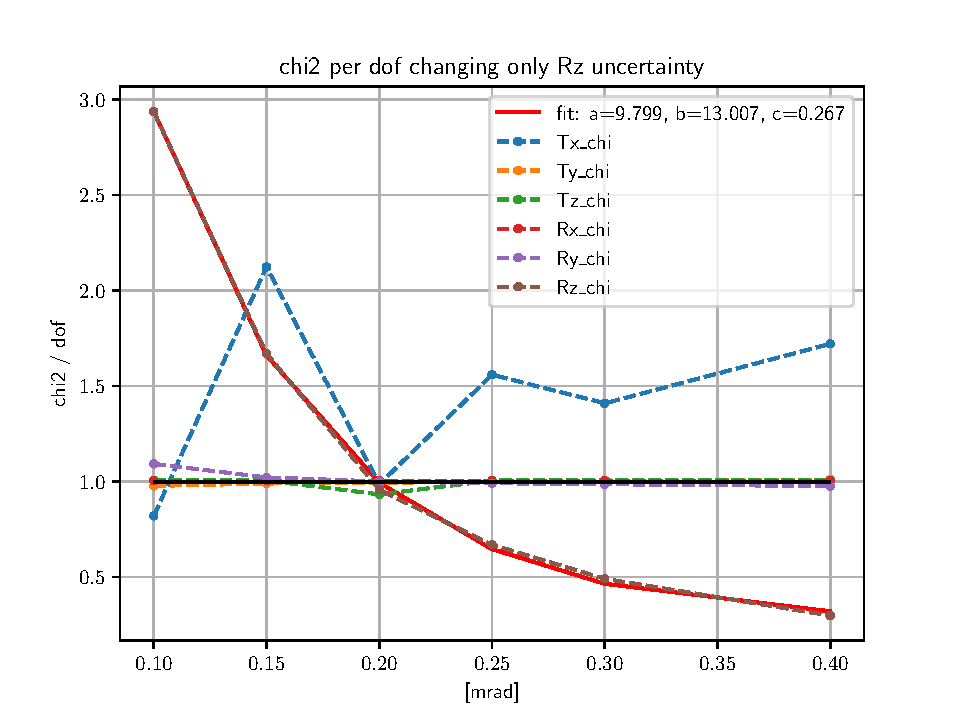
\includegraphics[width=\textwidth]{plots/retest/only_Rz_variable_full_fit.pdf}
%         \end{figure}
%       \end{column}
%   \end{columns}
% \end{frame}

% \begin{frame}\frametitle{Loose particle selection}
%   \begin{columns}
%     \begin{column}[c]{\textwidth}
%       \begin{itemize}
%         \setlength\itemsep{0em}
%         \item $\bullet$\, Same procedure performed for looser particle selection for V0 \to more events for mass peak analysis
%         \item $\bullet$\, tuned parameters for loose selection [$\mu m$,$\text{mrad}$]: 0.0074 1.2 1.9 0.4 0.00044 0.22
%         \item $\bullet$\, What does that mean for the joint constraint?
%         \begin{itemize}
%           \item $\bullet$\, Constraint is mainly influenced by $\textbf{Rx}$ and $\textbf{Tz}$ \to logical since this is the bending direction
%           \item $\bullet$\, $\textbf{Tx}$ (left-to-right movement) is basically fixed since it has no impact on the constraint, same for $\textbf{Ry}$ (rotation around vertical axis)
%         \end{itemize}
%       \end{itemize}
%     \end{column}
%   \end{columns}
% \end{frame}

% \begin{frame}\frametitle{What else did i do since DPG 2023 in march?}
%   \begin{itemize}
%     \item $\bullet$\, stability measurements
%     \item $\bullet$\, joint constraint analysis
%     \item $\bullet$\, from Alignment V10 for FSP to V8 today (not all of it is my work but i laid the foundation)
%     \item $\bullet$\, plots: 
%     \item $\bullet$\, stability (take from 108th lhcb week repo)
%     \item $\bullet$\, module joints (same repo but different input files, obviously)
%     \item $\bullet$\, maybe mention alignment v8 but i think the 2 new topics will fill the rest of the pages that i want to show
%     \item $\bullet$\, look at my slides from LHCb where i presented!!
%   \end{itemize}
% \end{frame}

\begin{frame}\frametitle{Summary}
  % >>> editors note: this summary/conclusion has to be changed to account for new findings with alignment v8, 
  % joint constraint analysis and stability tests for alignment runs
  \begin{itemize}
    \setlength\itemsep{0em}
    \item $\bullet$\, Source of complications: SciFi parts too far out of alignment to be correctly updated, corrected now with new alignment version and photogrammetry
    \item $\bullet$\, Adapt module positions by hand: working procedure for singular low-efficiency modules
    \item $\bullet$\, stability tests show no substantial difference in alignment quality from magnet polarity
    \item $\bullet$\, sufficient statistics: $150 \mu m$ movement; rerun manually if this is exceeded
    % \item $\bullet$\, Looser particle selection \to more events, residuals comparable to strict selection, better D0 mass peak
    % \item $\bullet$\, tuned parameters for loose selection [$\mu m$,$\text{mrad}$]: 0.0074 1.2 1.9 0.4 0.00044 0.22
    % \item $\bullet$\, What does that mean for the joint constraint?
    \begin{itemize}
      \item $\bullet$\, Constraint is mainly influenced by $\textbf{Rx}$ and $\textbf{Tz}$ \to logical since this is the bending direction
      \item $\bullet$\, $\textbf{Tx}$ (left-to-right movement) is basically fixed since it has no impact on the constraint, same for $\textbf{Ry}$ (rotation around vertical axis)
    \end{itemize}
  \end{itemize}
  % \textbf{Thank you for your attention!}
\end{frame}

%\begin{frame}
%  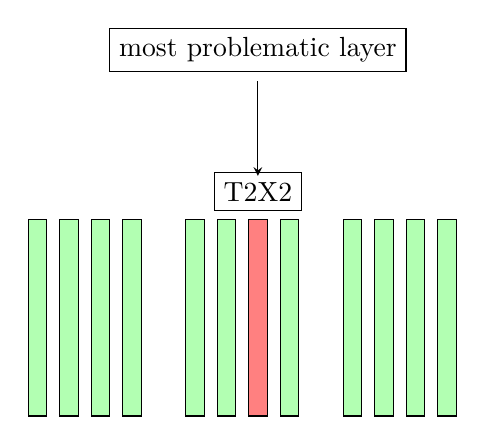
\begin{tikzpicture}

% first station
  \node[rectangle,
      draw = black,
      % text = ,
      fill = green!30!white,
      minimum width = 0.2cm,
      minimum height = 2.5cm] (r) at (0,0) {};

  \node[rectangle,
      draw = black,
      % text = ,
      fill = green!30!white,
      minimum width = 0.2cm,
      minimum height = 2.5cm] (r) at (0.4,0) {};

  \node[rectangle,
      draw = black,
      % text = ,
      fill = green!30!white,
      minimum width = 0.2cm,
      minimum height = 2.5cm] (r) at (0.8,0) {};

  \node[rectangle,
      draw = black,
      % text = ,
      fill = green!30!white,
      minimum width = 0.2cm,
      minimum height = 2.5cm] (r) at (1.2,0) {};

% second station
  \node[rectangle,
      draw = black,
      % text = ,
      fill = green!30!white,
      minimum width = 0.2cm,
      minimum height = 2.5cm] (r) at (2,0) {};

  \node[rectangle,
      draw = black,
      % text = ,
      fill = green!30!white,
      minimum width = 0.2cm,
      minimum height = 2.5cm] (r) at (2.4,0) {};

  \node[rectangle,
      draw = black,
      % text = ,
      fill = red!50!white,
      minimum width = 0.2cm,
      minimum height = 2.5cm] (r) at (2.8,0) {};
\node[draw, align=left] at (2.8, 1.6) {T2X2}; % node for bad layer
\draw[-stealth] (2.8,3.0) -- (2.8,1.8); % draw arrow to bad layer
\node[draw, align=left] at (2.8, 3.4) {most problematic layer}; % make node above layer

  \node[rectangle,
      draw = black,
      % text = ,
      fill = green!30!white,
      minimum width = 0.2cm,
      minimum height = 2.5cm] (r) at (3.2,0) {};

  % third station
    \node[rectangle,
        draw = black,
        % text = ,
        fill = green!30!white,
        minimum width = 0.2cm,
        minimum height = 2.5cm] (r) at (4,0) {};

    \node[rectangle,
        draw = black,
        % text = ,
        fill = green!30!white,
        minimum width = 0.2cm,
        minimum height = 2.5cm] (r) at (4.4,0) {};

    \node[rectangle,
        draw = black,
        % text = ,
        fill = green!30!white,
        minimum width = 0.2cm,
        minimum height = 2.5cm] (r) at (4.8,0) {};

    \node[rectangle,
        draw = black,
        % text = ,
        fill = green!30!white,
        minimum width = 0.2cm,
        minimum height = 2.5cm] (r) at (5.2,0) {};
\end{tikzpicture}

%\end{frame}

\begin{frame}\frametitle{Backup}
  $\textbf{Loose Tracking config and D0 selection}$
  \begin{columns}
    \begin{column}[c]{0.48\textwidth}
      \begin{figure}
        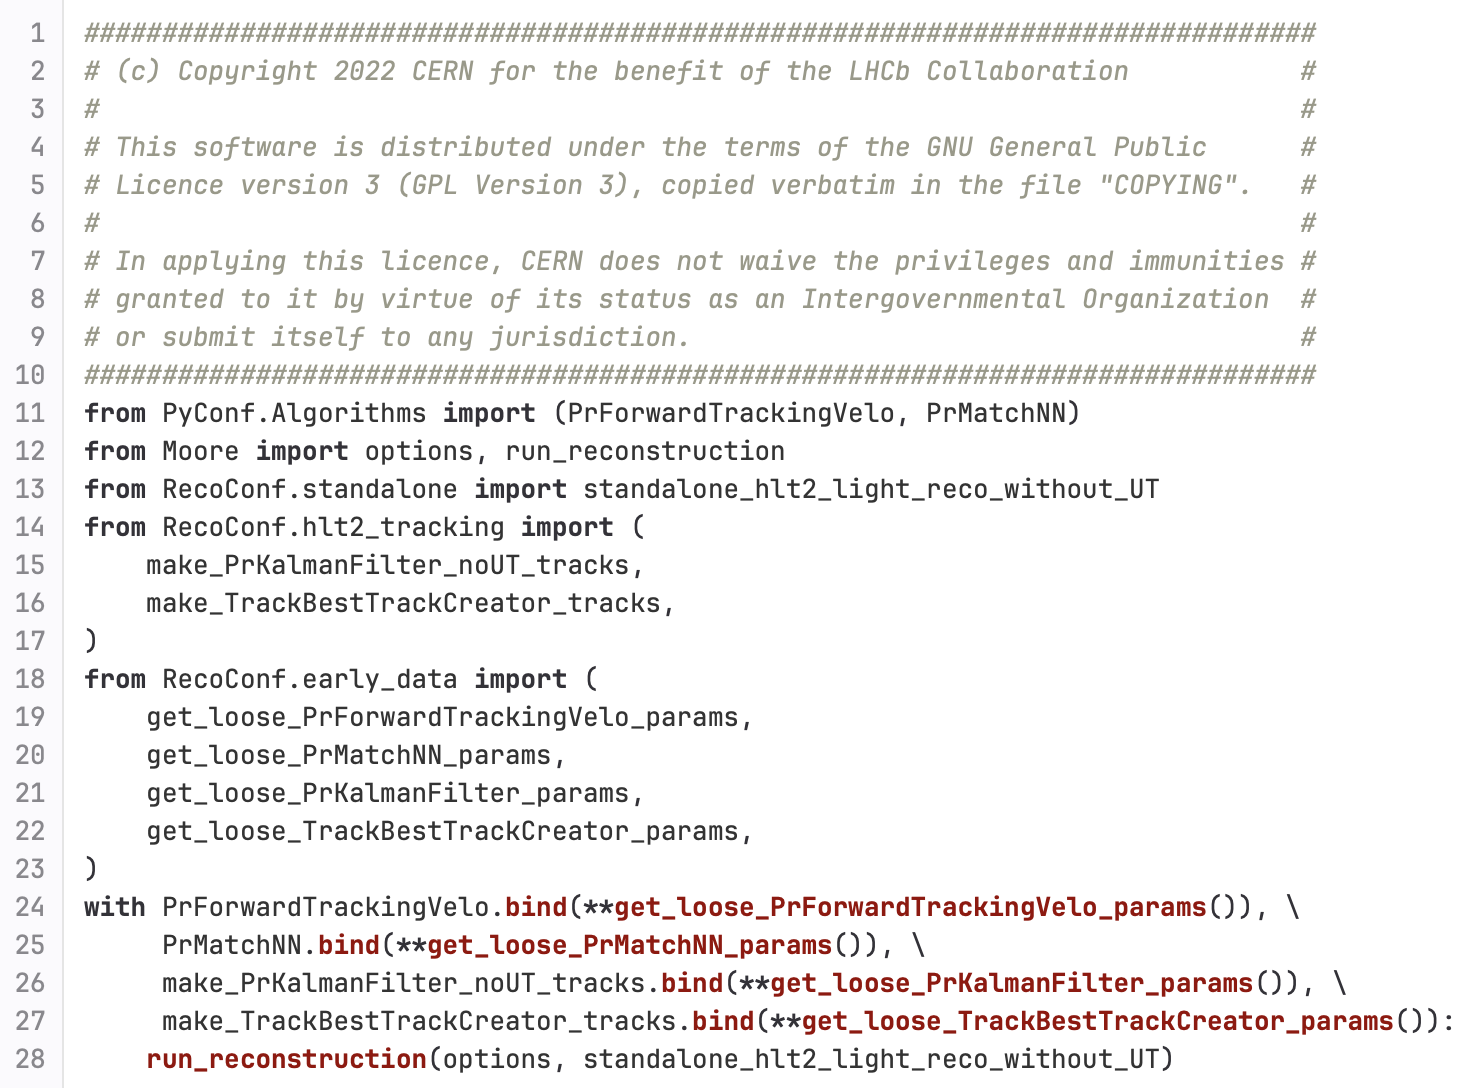
\includegraphics[width=\textwidth]{plots/loose_tracking.png}
      \end{figure}
    \end{column}
    \begin{column}[c]{0.48\textwidth}
      \begin{itemize}
        \item $pt_\text{min}$ = 800 MeV
        \item pion, kaon required to have min pt and IPCut = 60 $\mu m$
        \item mass hypothesis [1760 MeV, 1960 MeV]
        \item vertex $\chi^2$ < 10
      \end{itemize}
    \end{column}
  \end{columns}
\end{frame}

\begin{frame}\frametitle{Backup: stability dataset}
  % describe what loose tracking is!
  \begin{columns}
    \begin{column}[c]{0.9\textwidth}
      \begin{itemize}
        \setlength\itemsep{0em}
        \item $\bullet$\, Dataset contains magnet-up and magnet-down samples from 2022 labeled as "good" from EMTF
        \item $\bullet$\, Good: > 90\% of datalinks are good
        \item $\bullet$\, Includes runs from fills: 8489, 8491, 8496
        \item List of randomly chosen runs: 255949, 256030, 256145, 256159, 256163, 256272, 256278, 256290
        \item $\bullet$\, V3 Alignment from tag (loose tracking, half module alignment TxTz + Mat alignment, back layer fixed) from conditions database % backlayer fixed becasue q/p biggest influence and we want to fix this in place 
      \end{itemize}
    \end{column}
  \end{columns}
\end{frame}


% not needed
% \begin{frame}\frametitle{Sources}
%   \begin{itemize}
%     \item $\bullet$\,SciFi Conference Talk: \url{https://twiki.cern.ch/twiki/pub/LHCb/SciFiConference/fee_2018.pdf}
%     \item $\bullet$\,LHCb SciFi: From performance requirements to an operational detector: \url{https://indico.cern.ch/event/1163878/}
%     \item $\bullet$\, BCAM \url{https://accelconf.web.cern.ch/ipac2018/papers/wepaf067.pdf}
%   \end{itemize}
% \end{frame}

\end{document}
